\documentclass[12pt,a4paper]{article}
\usepackage[utf8]{inputenc}
\usepackage{indentfirst}
\usepackage[brazilian]{babel}
\usepackage{graphicx}
\usepackage{listings}
\usepackage{listingsutf8}
%\usepackage{hyperref}
\usepackage{url}
\usepackage[T1]{fontenc}
\usepackage{spverbatim}
\usepackage[top=2cm, bottom=2cm, left=2.5cm, right=2.5cm]{geometry}
\usepackage{fancyvrb,graphicx, color}
\usepackage{tabularx}
\usepackage{array}
\usepackage{cite}
\usepackage{subfigure}

\begin{document}
    \definecolor{aquamarine}{rgb}{0.5, 1.0, 0.83}
     % capa
\begin{titlepage}
\begin{center}
\begin{figure}[!htpb]
        \centering
        
\includegraphics[width=5em]{logo/logoUnB.jpg}
\end{figure}
{\large Universidade de Brasília}\\[0.2cm]
{\large Instituto de Ciências Humanas}\\[0.2cm]
{\large Departamento de Geografia}\\[4.1cm]
%{\bf RESENHA}\\
%{\bf Controle 6}\\
{\bf \huge  Analise Temporal da Região da Cidade de Manaus/AM.}\\[4.1cm]
\end{center}
{\large Aluno(a): Nelson dos Santos Luz - 10/0060323}\\[0.7cm]
{\large Professor(a): }\\[4.1cm]
\begin{center}
{\large BRASÍLIA/DF}\\[0.2cm]
{\large 14 Out 2015}
\end{center}
\end{titlepage}
	\newpage
    % Folha de rosto sem o uso de \folhaderosto
\begin{titlepage}
    \begin{center}
        {\large UNIVERSIDADE DE BRASÍLIA} \\
        {\large DEPARTAMENTO DE GEOGRAFIA} \\[3.3cm]
        {\large Nelson Dos Santos Luz} \\[3.3cm]
        {\Huge Analise Temporal da Região da Cidade de Manaus/AM.} \\[3.6cm]
        \hspace{.45\textwidth} % posicionando a minipage
        \begin{minipage}{.5\textwidth}
            %\begin{espacosimples}
                Trabalho final da disciplina de Fotointerpletação Aplicada ao Planejamento Urbano, Ministrada pelo Prof. Doutor .
            %\end{espacosimples}
        \end{minipage}\\[3.3cm]
        \vfill
        {\large BRASÍLIA} \\
        {\large 2015}
    \end{center}
\end{titlepage}
    \newpage
    \tableofcontents    
    \newpage
    \section{Introdução}
    \hspace{1.5cm}
    \section{Descrição da região de Análise}
    \subsection{Histórico}
\hspace{1.5cm}
Segundo o site da Prefeitura, a cidade de Manaus tem sua criação no século XVII para no primeiro momento demonstrar e fixar a presença portuguesa na região amazônica. Tem seu núcleo urbano, localizado na margem esquerda do Rio negro, teve início com a construção do Forte da Barra de São José no ano de 1669. Ao redor do Forte de São José do Rio Negro se desenvolveu o povoado do Lugar da Barra, que por conta da sua posição geográfica passou a ser sede da Comarca do São José do Rio Negro. Em 1755, por meio de Carta régia, a antiga missão de Mariuá foi escolhida como capital, passando a se chamar vila de Barcelos, anos mais tarde a sede foi transferida para o Lugar da Barra, que em 1832 tornou-se Vila da Barra, e em 24 de outubro de 1848, a Cidade da Barra de São José do Rio Negro. No entanto, com a elevação da Comarca à categoria de Província, em 1850, a Cidade da Barra, passou a se chamar em 04 de setembro de 1856, Cidade de Manaus, tornando-se independente do Estado do Grão-Pará. O nome lembra a tribo indígena dos Manáos, que habitavam a região onde hoje é Manaus antes de serem extintos por conta da civilização portuguesa, e seu significado é “mãe dos deuses”.\\

\hspace{1.5cm}
A cidade de Manaus viveu o surto da economia gomífera, de 1870 à 1913. Com a da perda do mercado mundial para a borracha asiática, a mesma retornou a um novo período de isolamento até o advento da Zona Franca de Manaus, em 1970. Segundo PNUD (2013)\cite{pnud2013}, entre os anos de 2000 e 2010, seu crescimento populacional foi numa taxa de 2,51\% anualmente. Neste período sua taxa de urbanização foi de 99,36\% para  99,49\%.  
    \section{Metodologia}
    \subsection{Aquisição}
\hspace{1.5cm}
A aquisição das imagens se deu junto ao catalogo do Instituto Nacional de Pesquisa Espacial (INPE). Foram adquirido imagens do LAndsat 5, respectivamente 1999 e 2011, da cidade de Manaus-AM. A figura \ref{Aquisição1}, mostra o processo de escolha da região de interesse. Neste caso foi escolhido a região da cidade de Manaus-AM.\\
\begin{figure}[!htpb]
        \centering
        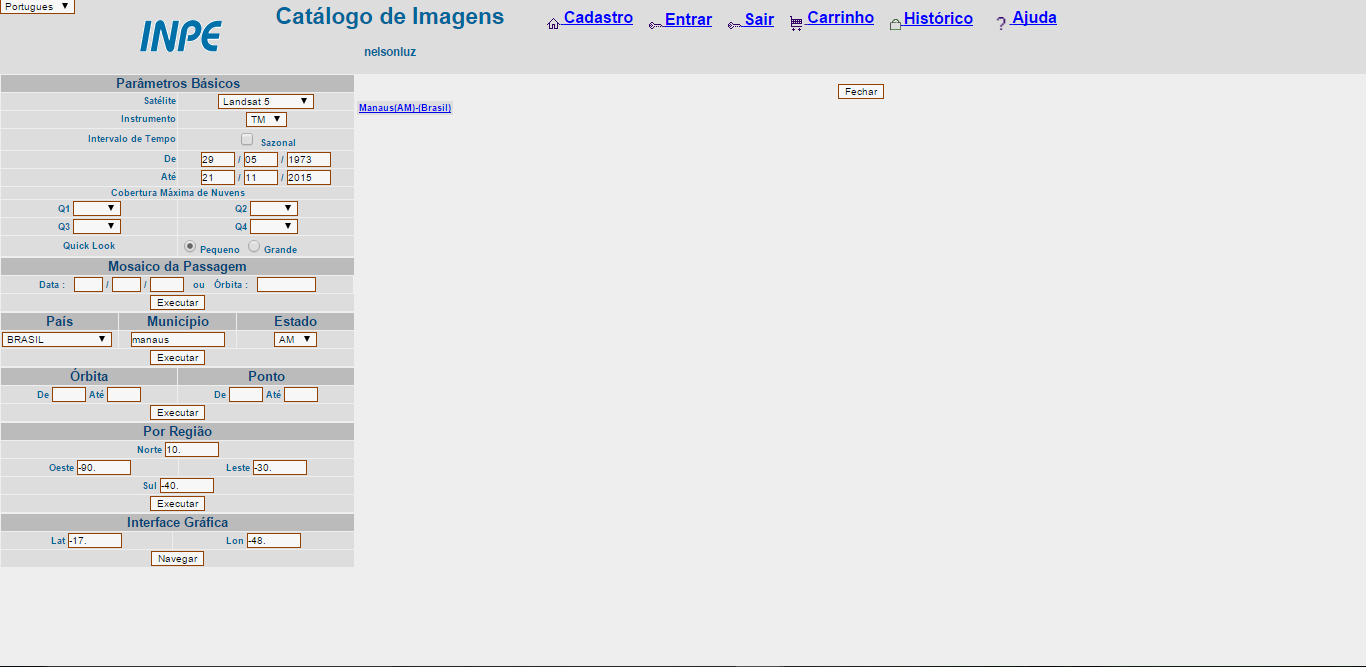
\includegraphics[scale=0.3]{imagens/aquisicao.png}
        \caption{site do INPE - Escolha da área de interesse.}
        \label{Aquisição1}
\end{figure}

\hspace{1.5cm}
Após a definição da área de estudo é necessário a seleção,figura \ref{Aquisição2}, da posição do satélite que melhor totalize a região estudada. As imagens da posição 231 melhor atendeu aos interesse, pois se tinha uma visão do todo da cidade.\\
\begin{figure}[!htp]
        \centering
        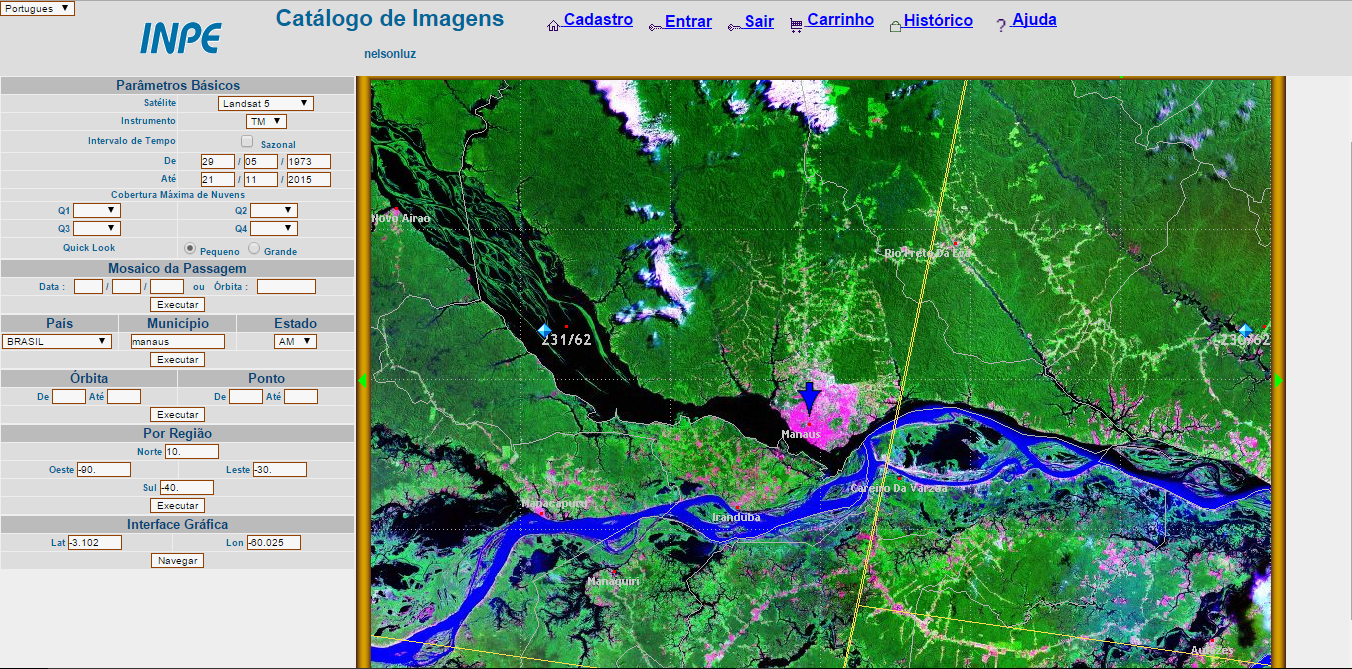
\includegraphics[scale=0.3]{imagens/aquisicao_02.png}
        \caption{site do INPE - Seleção da posição da imagens.}
        \label{Aquisição2}
\end{figure}

\hspace{1.5cm}
O INPE disponibiliza uma vasta coleção de imagens, do Landsat 5, compreendendo o período de 1984 a 2011. Dentro do seu catalogo, figura \ref{Aquisição3}, selecionamos e colocamos no carrinho as imagens que irá atender, nos seus respectivos anos. Foram selecionado os anos de 1999 e 2011, para se obter analise temporal de mais de 10 (dez) anos. \\
\begin{figure}[!htpb]
        \centering
        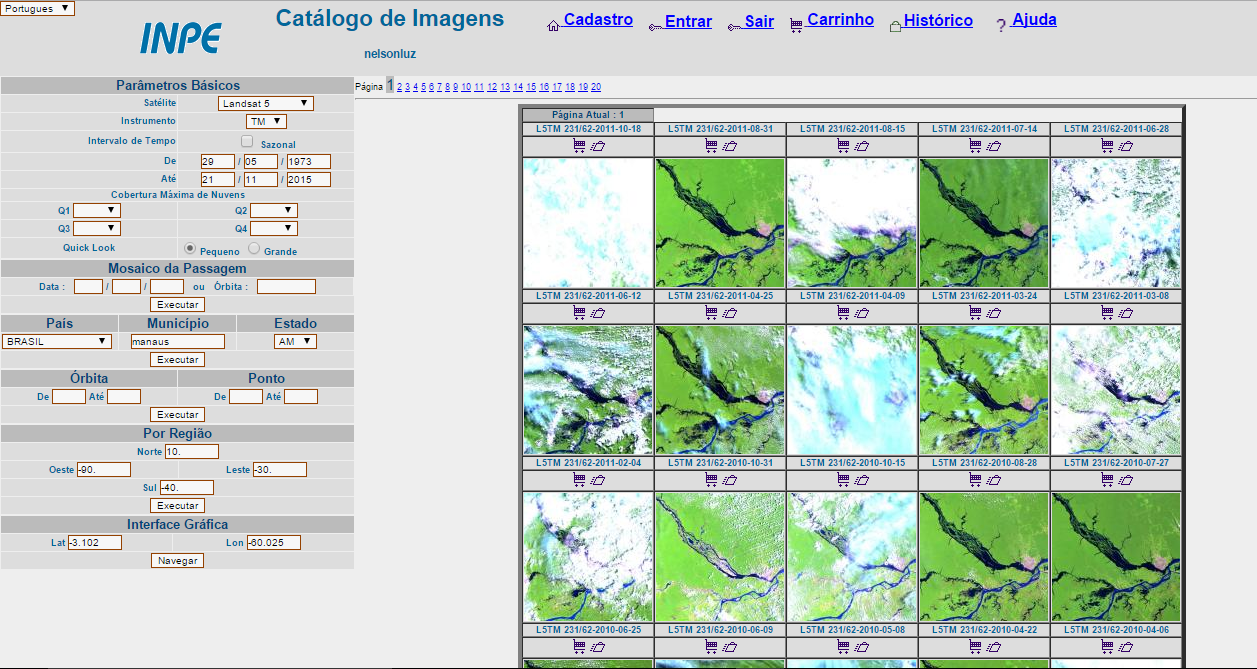
\includegraphics[scale=0.3]{imagens/aquisicao_03.png}
        \caption{site do INPE - Colocação das imagens selecionadas no carrinho.}
        \label{Aquisição3}
\end{figure}
\hspace{1.5cm}
As Imagens selecionadas são disponibilizadas através de um link "ftp", disponibilizado pelo INPE e enviado ao email do usuário cadastro no sistema.
\subsection{Calibração Radiométrica}
\hspace{1.5cm}
A Calibração Radiométrica é aplicada para imagens do tipo ASTER, AVHRR, MSS, QuickBird, TM and TIMS, com vista a realizar a técnicas de correções atmosférica. As imagens adquiridas foram do Landsat 5 TM, que foram calibradas pelo \textbf{\textit{Landsat TM Calibration}}, do programa Envi 4.7. A calibração se deu em todas as Bandas baixadas, excetuando a banda 6, do anos de 1999 e 2011. Processo foi realizado individualmente, para as 12 (dozes) bandas.

\hspace{1.5cm}
O processo de calibração ocorreu da seguinte forma:
\begin{itemize}
\item \textbf{Basic Tools}
\begin{itemize}
\item \textbf{Preprocessing  $\rightarrow$  Calibration Utilities  $\rightarrow$  Landsat TM}.\\
\end{itemize}
\begin{figure}[h!]
\centering
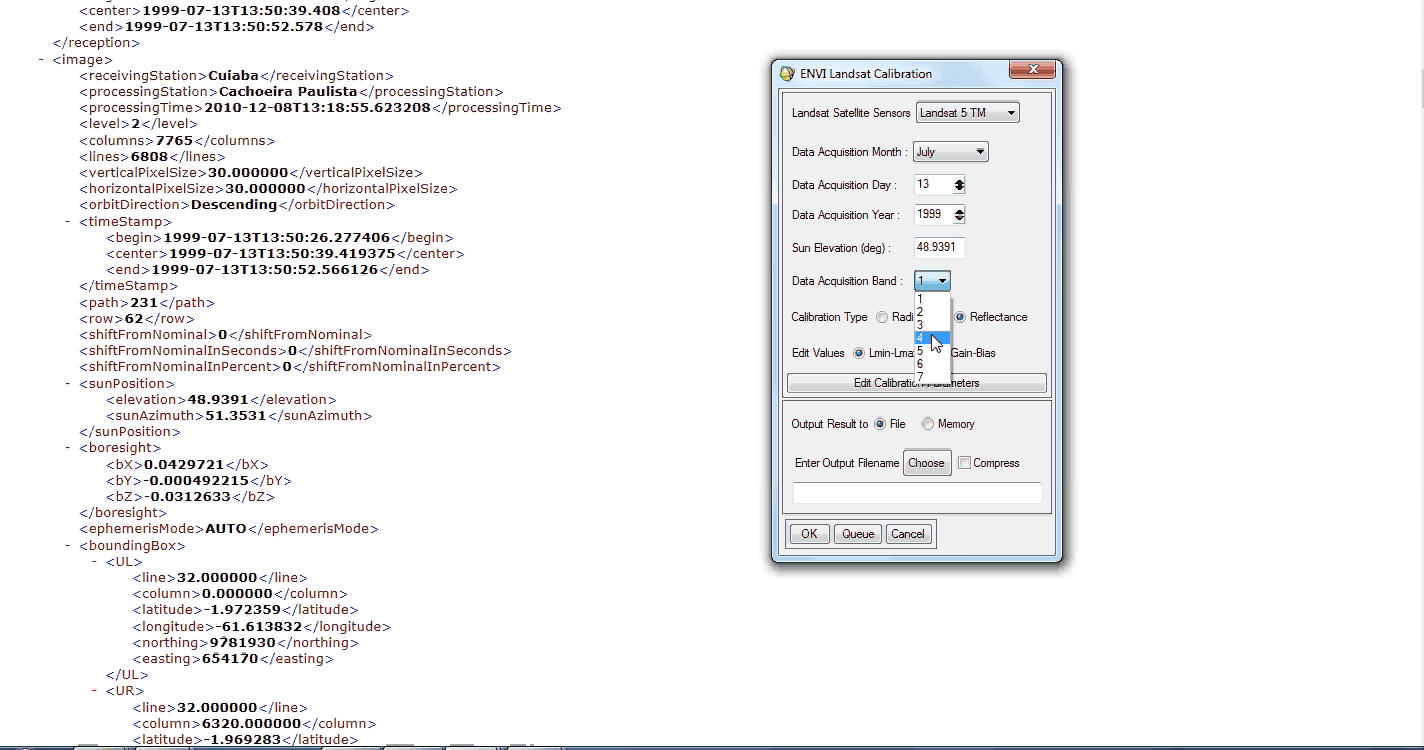
\includegraphics[scale=0.3]{imagens/calibracao03.png}
\caption{Configuração para calibração das imagens.}
\label{calibracao03}
\end{figure}

\end{itemize}
\hspace{1.5cm} Na janela \textbf{\textit{TM Calibration Parameters}} é selecionado o tipo de satélite, no nosso caso \textit{Landsat 5}; Mês de aquisição da imagem, no primeiro conjunto  08 e no segundo 10; dia de aquisição da imagem, no primeiro conjunto  13 e no segundo 23; Ano de aquisição da imagem, no primeiro conjunto  1999 e no segundo 2011;e Sun Elevation, em cada banda (figura ) foi adquirido um grau diferente, dentro de um arquivo XML (figura \ref{calibracao03}).
Após o procedimento escolhe o tipo de saída do resultado: \textbf{Arquivo} e salva.
\subsection{Corte}
\hspace{1.5cm}
Para uma distribuição e visualização da área de estudo é necessário realizar o recorte da mesma. Este processo é necessário para um bom trabalho, no processo digital de imagens. Isto faz com que o estudo se der somente na área de interesse do pesquisador. 

\begin{itemize}
\item \textbf{Basic Tools}
\begin{itemize}
\item \textbf{Layer Stacking} $\rightarrow$ \textbf{Spatial Subset}\\

\end{itemize}
\begin{figure}[!htpb]
        \centering
        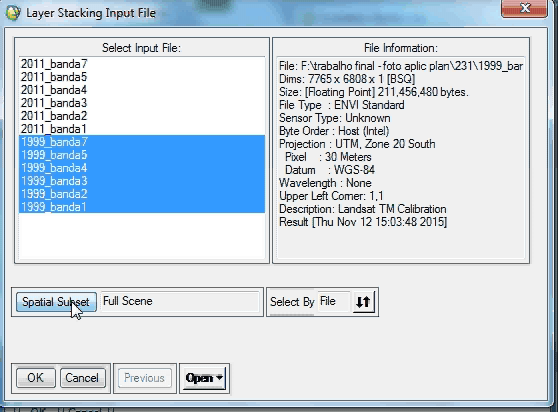
\includegraphics[scale =0.4]{imagens/corte04.png}
        \caption{Escolha dos Bandas para corte.}
        \label{corte04}
\end{figure}
\begin{figure}[!htpb]
        \centering
        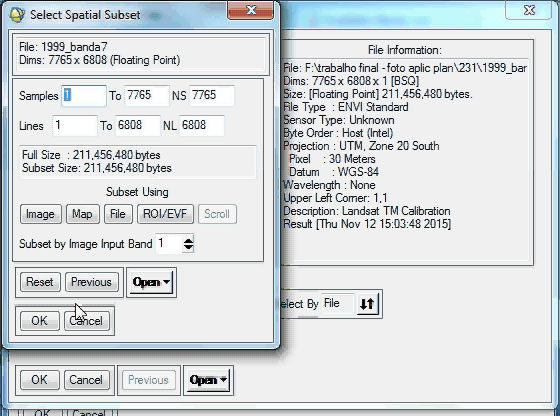
\includegraphics[scale=0.4]{imagens/corte05.png}
        \caption{Escolha dos Bandas para corte.}
        \label{corte05}
\end{figure}
\begin{figure}[!htpb]
        \centering
        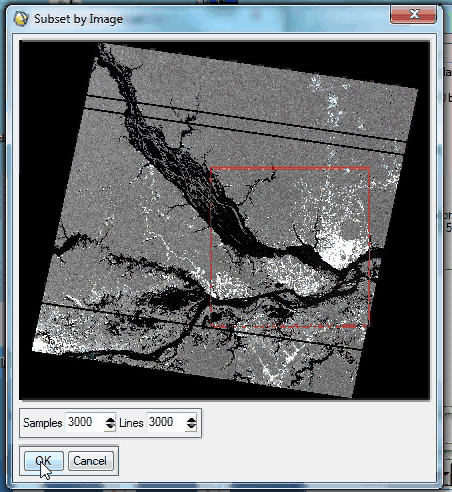
\includegraphics[scale=0.5]{imagens/corte06.png}
        \caption{Marcação da área para o corte.}
        \label{corte06}
\end{figure}
\end{itemize}
\hspace{1.5cm} Na figura \ref{corte04}, temos a escolha das bandas. A janela, figura \ref{corte05}, \textbf{Select Spatial Subset}, no primeiro momento escolhemos a opção \textbf{imagem} (figura \ref{corte06}). Já para realizá o a marcação das outras bandas utilizamos a opção \textbf{File} demonstra como foi feito o processo. O empilhamento é executado junto com o corte, na sequência.
\subsection{Empilhamento das Bandas}
\hspace{1.5cm}
Segundo o ENVI\cite{envi}, este sistema é usado para construção de um novo arquivo com imagens georeferenciada. As bandas são reamostradas e re-projetada em projeções e tamanho de pixel compativeis. Todas as imagens são compactadas em um unico arquivo, o facilita a manipulação das mesma. 

\begin{itemize}
\item \textbf{Basic Tools}
\begin{itemize}
\item\textbf{ Layer Stacking}\\

\end{itemize}
\begin{figure}[!htpb]
        \centering
        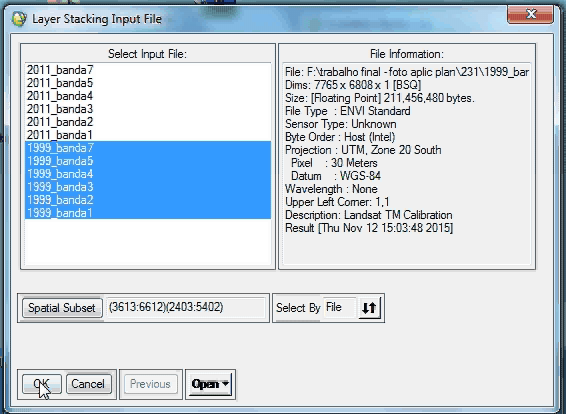
\includegraphics[scale=0.4]{imagens/empilhamento01.png}
        \caption{Escolha dos arquivos para empilhamento.}
        \label{empilhamento01}
\end{figure}        
\begin{figure}[!htpb]        
        \centering
        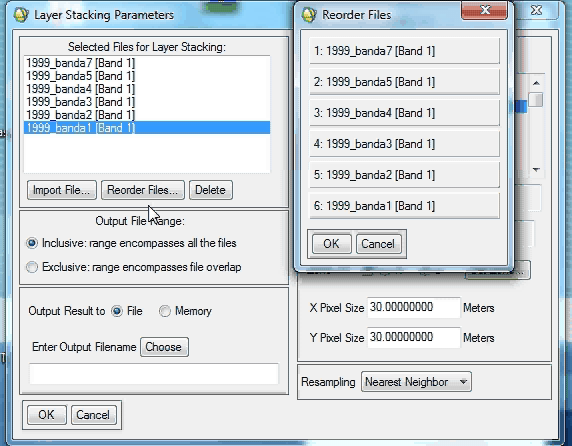
\includegraphics[scale=0.4]{imagens/empilhamento03.png}
        \caption{Reordenação das Bandas.}
        \label{empilhamento03}
\end{figure}        
\begin{figure}[!htpb]        
        \centering
        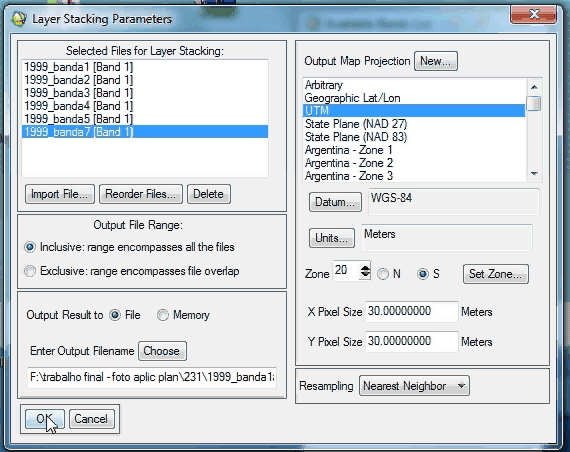
\includegraphics[scale=0.4]{imagens/empilhamento05.png}
        \caption{Nome do arquivo com as Bandas.}
        \label{empilhamento05}
\end{figure}
\end{itemize}
\hspace{1.5cm}
Depois de corte das imagens na tela de parâmetros com as bandas já selecionadas, clica no botão \textbf{Import File}, conforme figura \ref{empilhamento01}.Na próxima janela é necessário a reordenação das imagens, através do botão \textbf{Reorder Files}, figura \ref{empilhamento03}. Depois escolher o local/nome do arquivo e realizar a criação do empilhamento das bandas, figura \ref{empilhamento05}. 

\subsection{Correção Geométrica}
\hspace{1.5cm}
Para ENVI \cite{envi}, realizar a analise temporal de duas imagens é necessário construir a correção geométrica. Isto processo tem fundamental devido aos acidentes geográfico não estarem sobreposto nas imagens. Este metodo basea-se em marcar os pontos de controles nos acidentes, nas duas imagens (imagem-to-imagem).\\

\begin{itemize}
\item Map
\begin{itemize}
\item \textbf{Registration} $\rightarrow$ \textbf{Select GCPs:Image to Image}
\end{itemize}
\begin{figure}[!htpb]
        \centering
        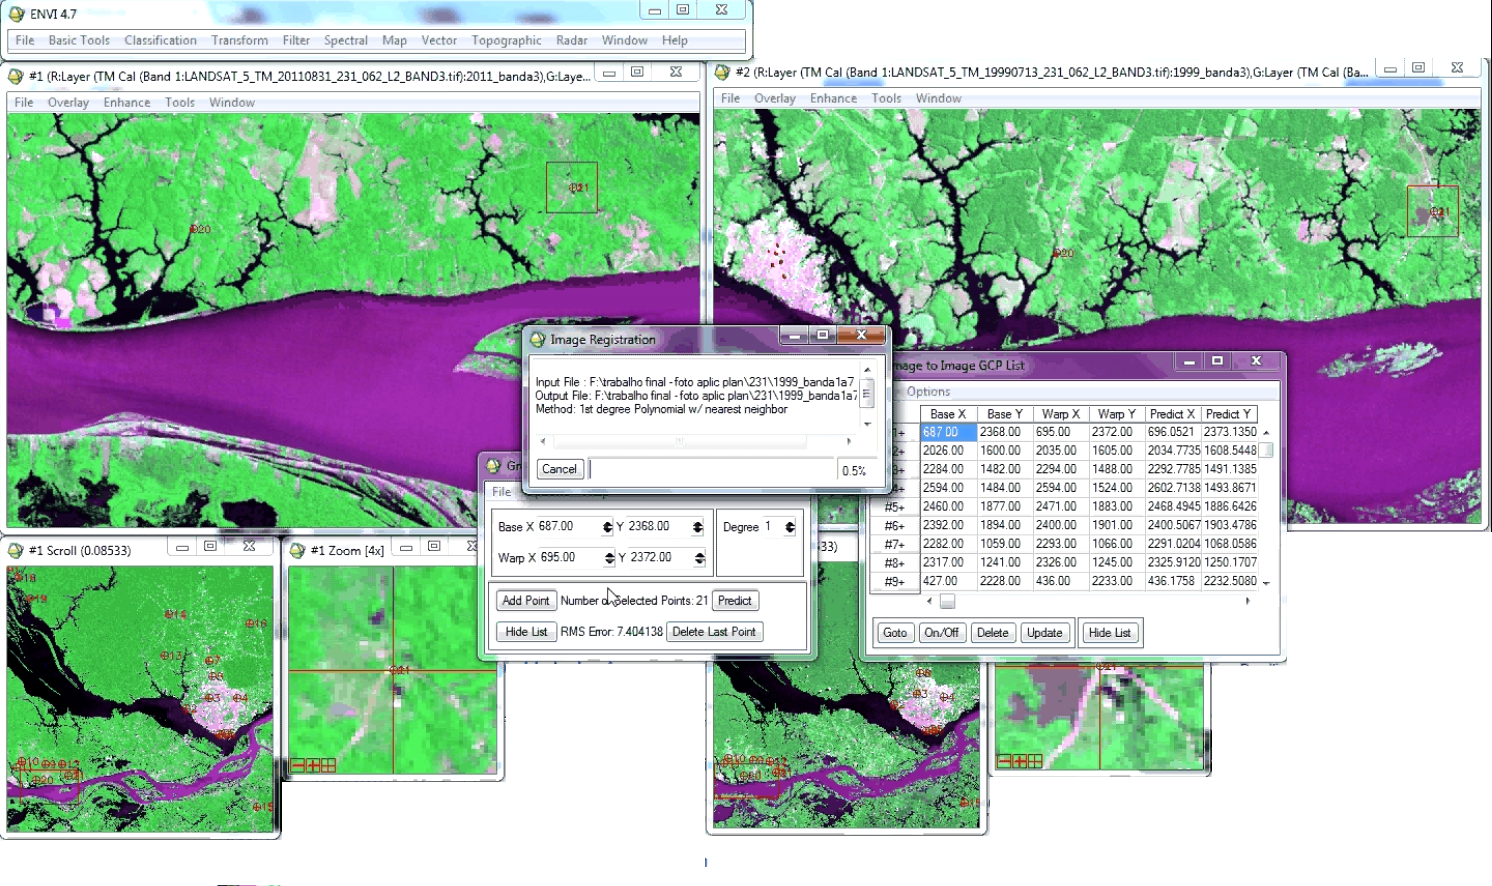
\includegraphics[scale =0.2]{imagens/correcao04a.png}
        \caption{Processo de Correção Geométrica.}
        \label{correcao04}
\end{figure}
\end{itemize}
\hspace{1.5cm}
No nosso processo foram selecionado 20 (vinte) pontos de controles, nas dois compostos de banda. Os pontos são melhores definidos na janela de zoom. Após a coleta de pontos nos acidentes é dado o nome do arquivo "pts" e chamado no \textbf{Map} $\rightarrow$ \textbf{Registration} $\rightarrow$ \textbf{Warp from GCPs:image to Image}, para gerar a correção entre a imagem (base e warp). A figura \ref{correcao04} mostra o processo realizado.


\subsection{Classificação}
\hspace{1.5cm}
Neste processo é extraído  as informações das imagens, com a finalidade de reconhecer padrões e objetos mapeando as áreas da superfícies terrestre. Na área de estudo foi utilizado as cores, como associação de classe (Água $\rightarrow$ \textcolor{blue}{Azul}, Água com sedimentos $\rightarrow$ \textcolor{aquamarine}{Aquamarine}, Vegetação $\rightarrow$ \textcolor{green}{Verde} e Urbanização $\rightarrow$ \textcolor{red}{Vermelho}). Este passo desenvolveu-se com a criação da \textbf{\textit{Region of Interess}} (ROI), conforme figura \ref{roi01}.
\begin{itemize}
\item \textbf{Basic Tools}
\begin{itemize}
\item \textbf{Region of Interess}\\
\item \textbf{Amostras}\\
\begin{tabular}{|c|c|c|}
\hline
Tipo & Polignos & Points\\
\hline
\colorbox{blue}{Água} & 22 & 1155 \\
\hline
\colorbox{aquamarine}{Água com sedimentos} & 23&1350\\
\hline
\colorbox{green}{Vegetação} & 22&1138\\
\hline
\colorbox{red}{Urbanização} \footnote{No processo foi considerado urbanização tanto as construções, bem como os solos expostos.} & 30&586\\
\hline
\end{tabular}
\end{itemize}
\begin{figure}[!htpb]
        \centering
        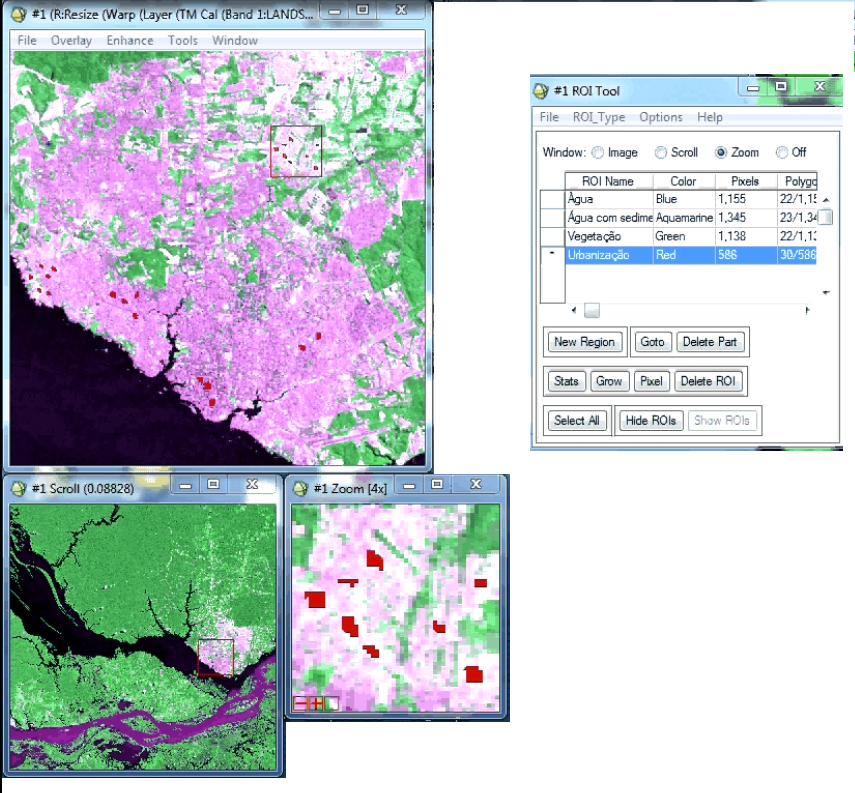
\includegraphics[scale =0.5]{imagens/roi01a.png}
        \caption{Geração das classes de Uso do Solo.}
        \label{roi01}
\end{figure}
\end{itemize}
\hspace{1.5cm}
Nosso processo de analise temporal será elaborado pelo modo supervisionado, mínima distancia. Este processo tem como primeira fase a coleta de amostra, das diversas classes. Aqui foi definido os tipos de classes do solo, para estudado, com suas respectivas cores.
\begin{itemize}
\item \textbf{Classification}
\begin{itemize}
\item \textbf{Supervised} $\rightarrow$ \textbf{Minimum Distance}\\
\end{itemize}
\begin{figure}[!htpb]
        \centering
        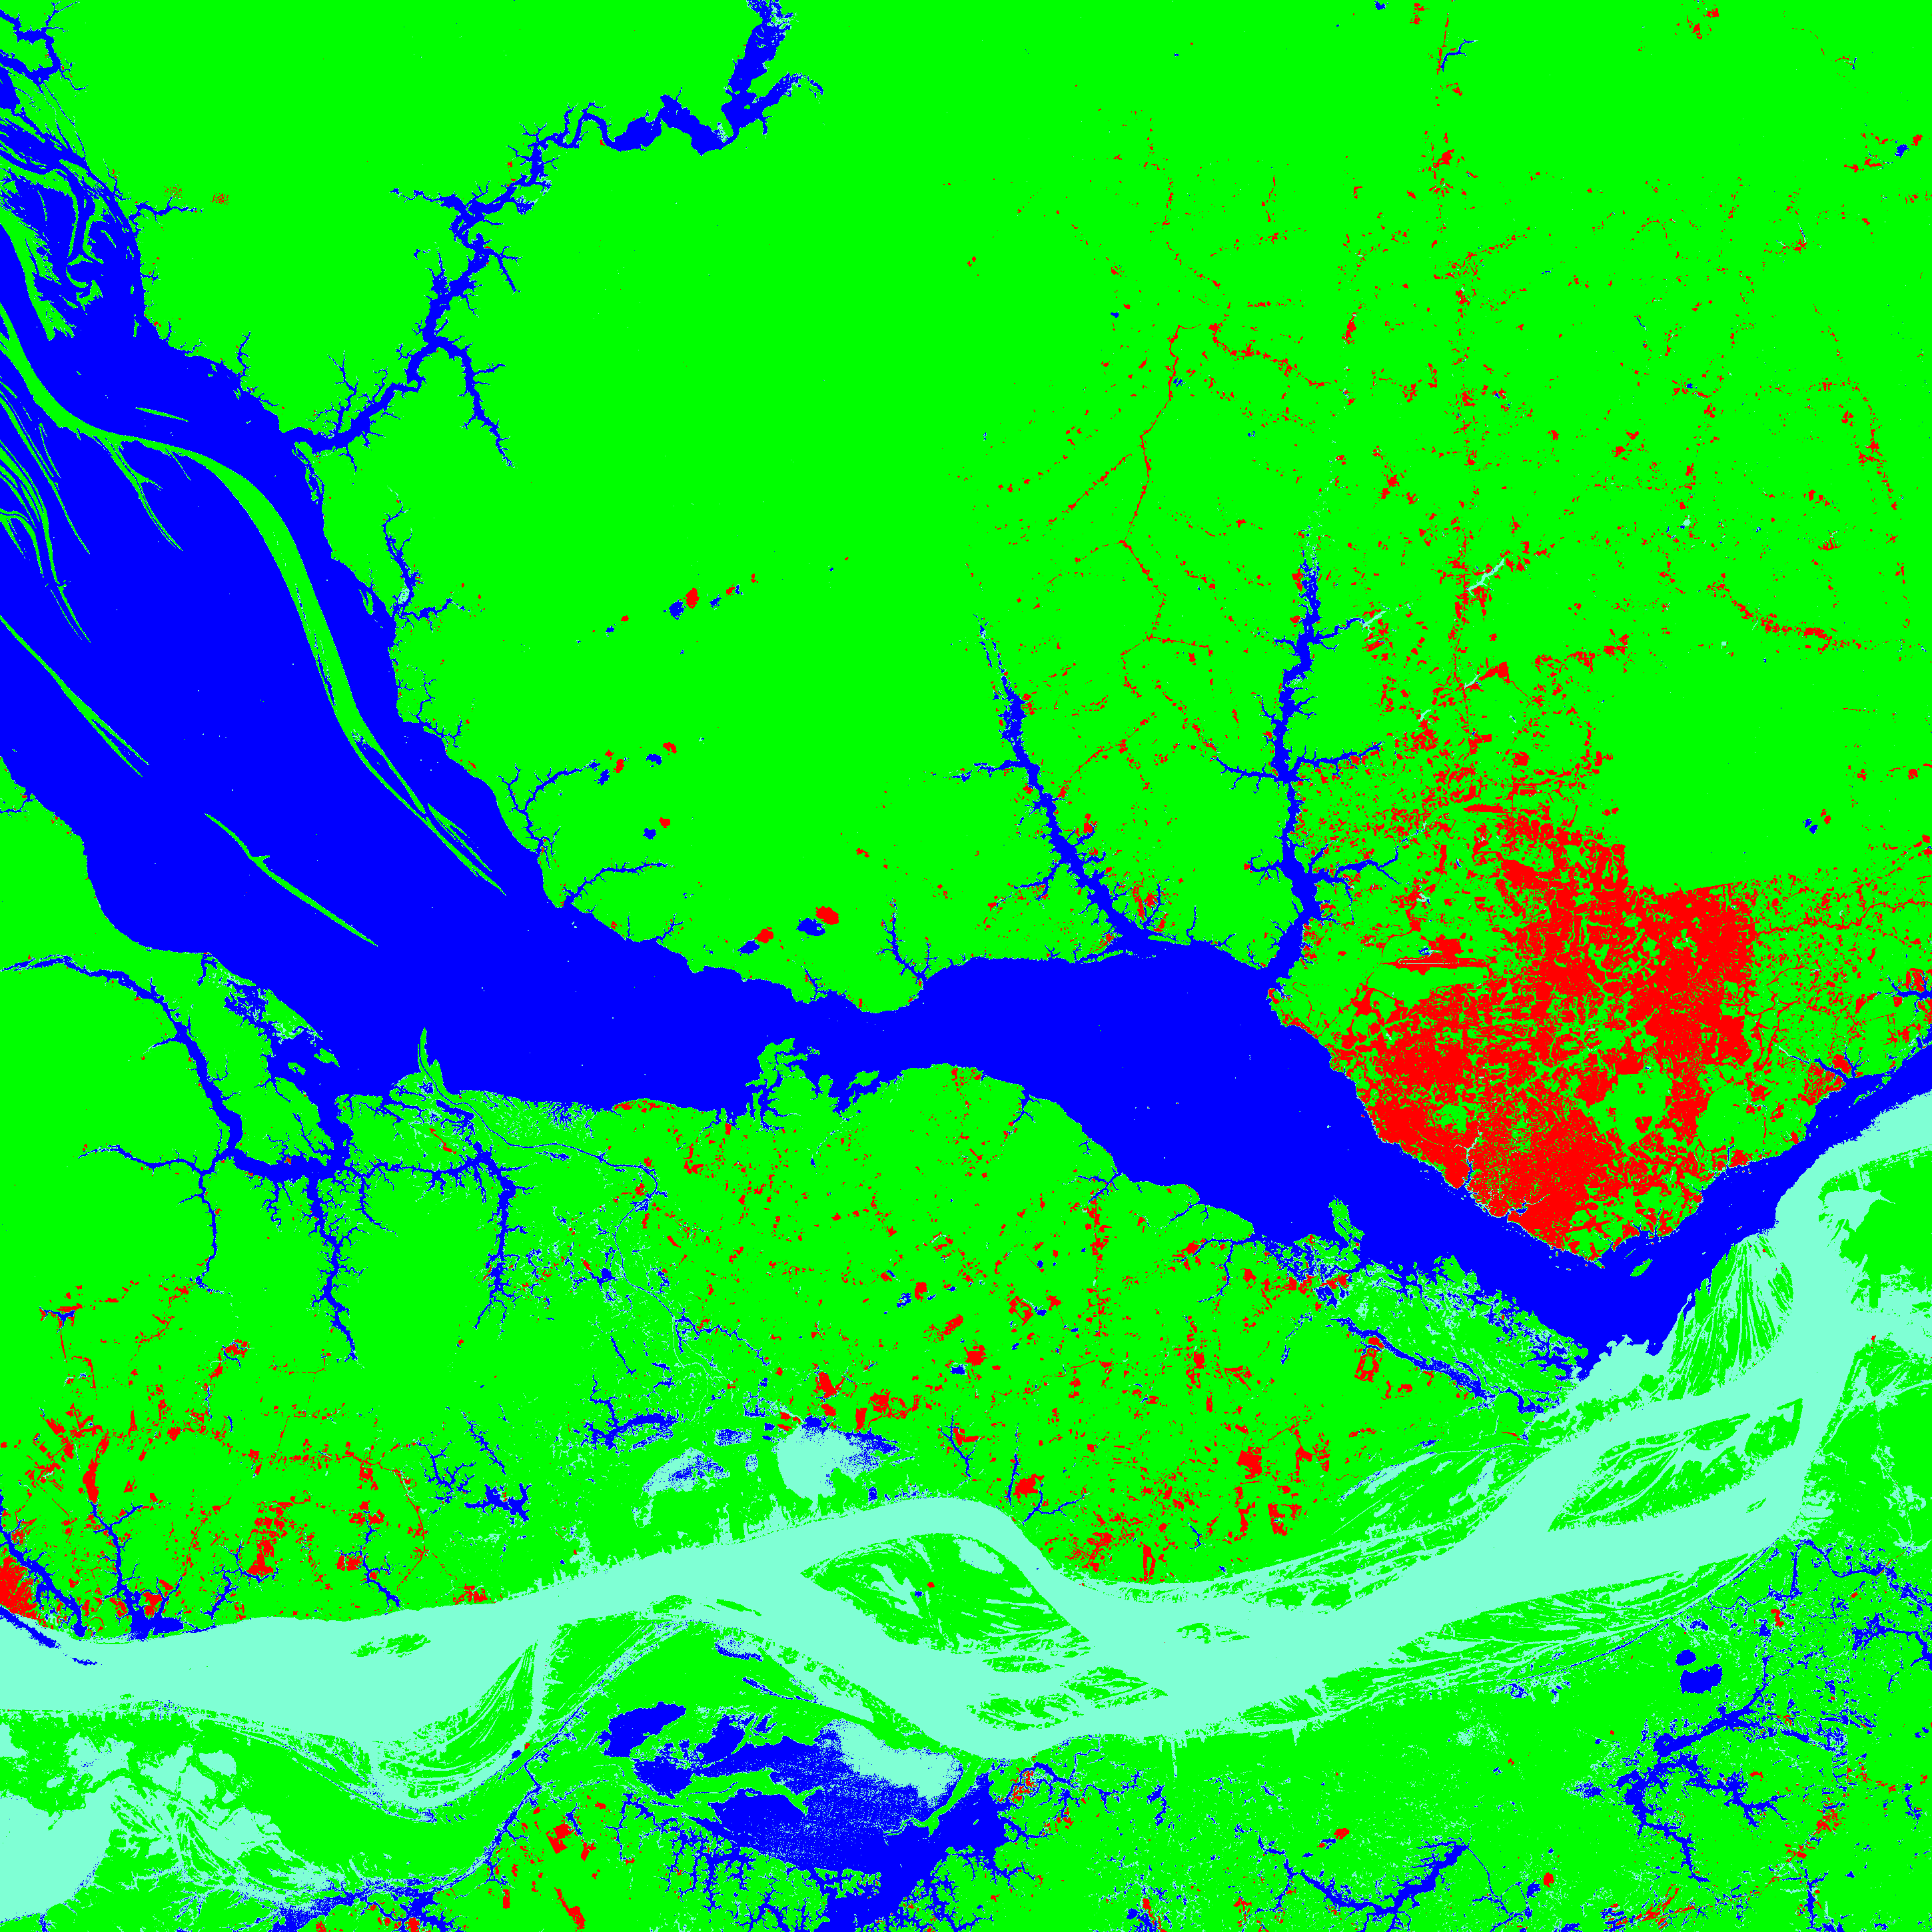
\includegraphics[scale =0.1]{imagens/1999_banda1a7_Class_MinDist.png}
        \caption{Geração das classes de Uso do Solo.}
        \label{1999}
        \centering
        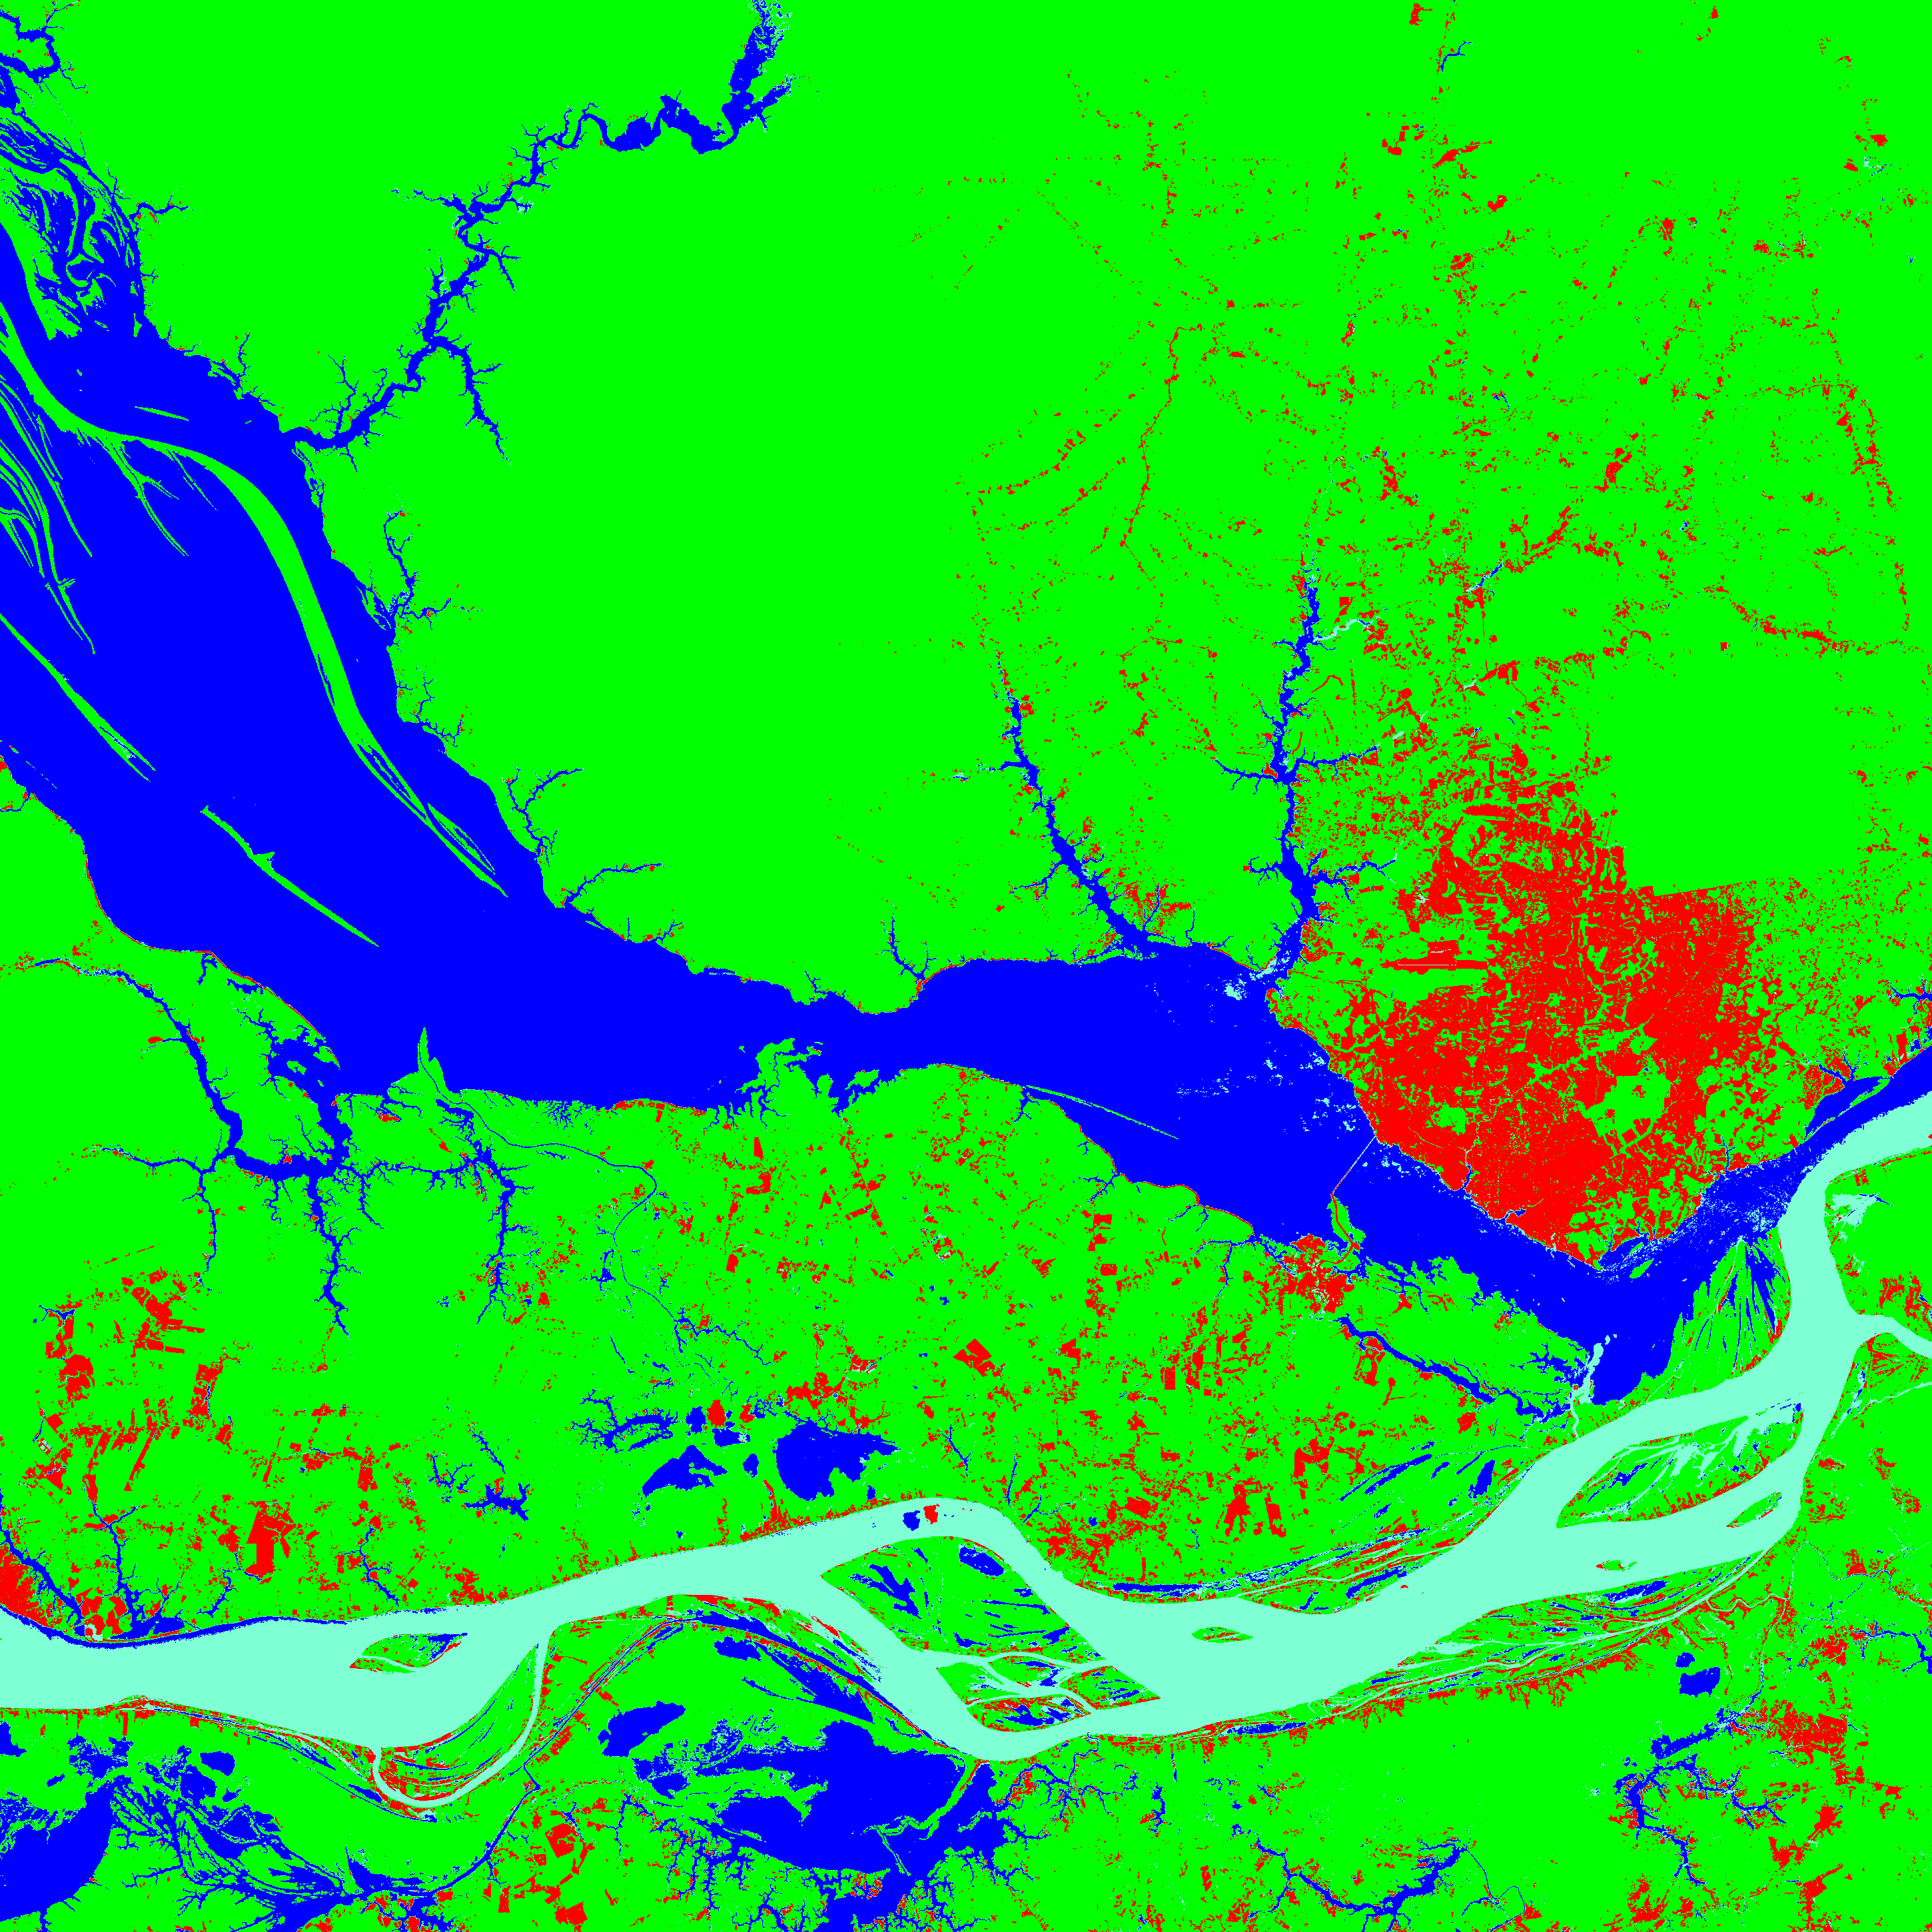
\includegraphics[scale =0.1]{imagens/2011_banda1a7_Class_MinDist.png}
        \caption{Geração das classes de Uso do Solo.}
        \label{2011}
\end{figure}
\end{itemize}
\hspace{1.5cm}
Esta técnica encontra os vetores desconhecido de cada classe, através dos calculos da distance Euclidean de cada vetor conhecido. Nas figuras ... e ... temos o resultado alcançado, para os anos de 1999 e 2011, respectivamente.


\subsection{Tabulação Cruzada}
\hspace{1.5cm}
A tabulação cruzada é realizada para a análise de dados. Nela temos a amostra dividida em subgrupos, para se poder verificar a respostas dentro dos grupos. No nosso caso foi gerado um arquivo de estaticas, partido das classificações feitas dos bandas.
    \section{Resultado}
    \hspace{1.5cm}
    \begin{thebibliography}{9}


%\bibitem{Erdos01} P. Erd\H os, \emph{A selection of problems and
%results in combinatorics}, Recent trends in combinatorics (Matrahaza,
%1995), Cambridge Univ. Press, Cambridge, 2001, pp. 1--6.

%\bibitem{ConcreteMath}
%R.L. Graham, D.E. Knuth, and O. Patashnik, \emph{Concrete
%mathematics}, Addison-Wesley, Reading, MA, 1989.

%\bibitem{Knuth92} D.E. Knuth, \emph{Two notes on notation}, Amer.
%Math. Monthly \textbf{99} (1992), 403--422.

\bibitem{pnud2013} PNUD, \emph{Programa das Nações Unidas para o Desemvolvimento },  Atlas do Desenvolvimento Humano no Brasil (2013), Disponível em 
\url{http://www.atlasbrasil.org.br/2013/pt/perfil_m/manaus_am}.

\bibitem{envi} ENVI, \emph{ENVI User’s
Guide
}, Version 4.1, 2004, Research Systems Inc.
\end{thebibliography}
    %\bibliographystyle{pain}
    %\bibliography{trabalho/ref_trab_foto}
\end{document}